% !TEX root = ../swputhesis.tex
\chapter{绪论}
\section{研究背景与意义}
长期以来,交通事故常常是由于人类驾驶员的错误操作而导致的,这给人们带来了人员伤亡和经济损失。为了解决这个问题,研究人员引入了自动驾驶的概念,旨在提高汽车乘员的安全性和舒适性\cite{秦飞巍2021无人驾驶中的场景实时语义分割方法}。自动驾驶是指在智能系统的控制下驾驶汽车,实现准确决策的智能系统需要具备场景理解的能力。全景分割技术可以作为一种出色的方法,因为从摄像头获取的图像需要经过处理才能理解场景\cite{everingham2010pascal}。

在这个领域,已经存在各种全景分割方法,其中一些试图在准确性和速度之间取得平衡。然而,正确识别对象边界内的像素标签和考虑不同比例的对象是两个具有挑战性的问题,使得这些架构难以达到高准确性。

语义分割是计算机视觉领域中的一项重要任务,其目标是将输入的图像分割成多个语义区域,并为每个像素分配一个语义标签,以确定其所属的语义类别。与传统的图像分割任务不同,语义分割需要对每个像素进行分类,而不仅仅是将图像分割成不同的区域。例如,在街景图像中,语义分割可以将图像分成道路、建筑、车辆、行人等多个语义区域,并为每个像素指定其所属的语义类别。语义分割在自动驾驶、物体识别、场景理解等领域具有广泛的应用。

实例分割是一种将目标检测和语义分割结合起来的技术,它仅针对图像中的目标进行检测,并对检测到的目标进行精细分割。与目标检测中的边界框相比,实例分割能够提供更精确的物体边缘信息\cite{kirillov2019panoptic}。
日常生活中发生着很多基于全景分割技术完成图像生成的应用,尤其是近年来蓬勃发展的自动驾驶车辆有关研究,在车辆行进过程中,自动驾驶技术首先获取到车辆、行人和其他移动物体信息,基于这些信息构建调控模型,再依据这些信息完成对车辆转向、刹车、速度的自动控制。目前汽车信息感知常用毫米波雷达和激光雷达,这些感知器将微波或激光发射到大气中后,接收障碍物反射的信号后进行处理,虽然这类技术具有较高的障碍物识别性能,但缺乏进一步提供车辆周围障碍物的分析能力,例如周围障碍物的大小和运动信息。为解决该问题,模仿人类使用触觉和视觉识别周围环境的模式,越来越多的自动驾驶技术在保留雷达感知技术的基础上,引入了前置摄像头增强车辆感知技术,通过对相机所得图像执行分割来增强驾驶环境信息。近年来,深度学习在计算机视觉领域的巨大发展,大大提升了机器实现图像识别的精度和性能,也很众多分类和全景分割网络神经网络\cite{wangye}被用于增强车辆自动驾驶的可靠性。图像的准确分割和理解建模已逐渐成为自动驾驶技术承上启下的关键调控技术,许多学者深耕于结合低耗时实现图像的高精度分割。

全景分割是将语义分割和实例分割相结合的技术,旨在对图像中的所有物体和背景进行检测和分割\cite{he2017mask}。与仅对感兴趣的目标区域进行分割的实例分割不同,全景分割需要对整个图像进行完整的分割,包括背景区域的分割。在全景分割中,背景区域的分割属于语义分割,而物体的分割则属于实例分割\cite{wu2019wider}。

图像分割主要有三种方式,即实例分割、语义分割和全景分割,它们之间存在一定的关联:
(1)实例分割:将图像中的每个对象分割出来,并将其转换为不同的实例。例如,在一张图像中有人和动物,可以将人和动物的轮廓分割成不同的实例\cite{he2017mask}。
(2)语义分割:将具有相同语义类型的图像区域分割成不同的区域,确保区域之间没有重叠。例如,对于街景图像,可以将道路、天空、建筑物等元素利用语义分割成多个区域\cite{long2015fully}。
(3)全景分割:对图像中每个像素的标签进行预测,并按照类别对像素进行分类,使得每个像素都有对应的语义类别。全景分割是语义分割和实例分割的综合称呼,在全景分割过程中,每个对象和像素都必须经过实例和语义分割才能预测标签。

总的来说,全景分割包括了实例分割和语义分割,如果能够同时预测每个像素的标签和实例编号,就能得到完整的全景分割图像。

当前主流的全景图像分割体系结构主要包括自上而下、自下而上和单径结构。自上而下的体系结构可以进一步划分为单相和双相模型\cite{he2017mask}。在自上而下的全景图像分割方法基础上,引入了一种新的图像分割方法。该方法采用两级图像分割模式,首先利用二级神经网络对一级图像进行后处理,然后再对一级图像进行后处理,实现全景图像的分割。为了减少自顶向下两阶段全景分割模型的计算复杂度,自顶向下单阶段全景分割模型省略了建议生成阶段,仅基于单阶段的目标检测来进行分割。此外,还采用了自下而上的方式,对原始影像中的每个像素进行义项分类,然后通过群组聚类的方式,在相同的义项下实现对不同样本的判别。无论是自上而下还是自下而上的全景图像分割算法,都是基于两条路径,即语义和实例路径,将物体与背景分离。而完整卷积单路径则将实例与背景的分割统一起来。

\section{全景分割图像生成}
在现实生活中,基于全景分割的图像生成应用非常广泛。例如,在自动驾驶领域,通过感知车辆、行人和移动物体等障碍物,来控制车辆的加速度。自动驾驶系统通过识别驾驶环境中的要素,如道路、车道、交通信号灯和标志,来确定车辆的行驶方向。为了实现准确的障碍物识别,汽车中使用的雷达和激光雷达可以发送微波或激光,并接收和处理障碍物反射的信号。然而,它们无法提供复杂的环境信息,如道路边界和车道分类。为了获取更详细的驾驶环境信息,前置摄像头成为必要的传感器之一,它通过处理图像来提供驾驶环境信息,就像人们通过视觉来认知周围环境一样。近年来,深度学习的发展极大地提升了图像识别性能,因此被应用于对车辆的高可靠性需求中的分类和全景分割网络。

对图像的准确理解和建模一直以来都备受关注,因为精确的场景模型是实现智能安防和自动驾驶等高层任务的基础。目前,像素级的场景理解主要包括实例分割和语义分割,而全景分割作为一种新提出的技术,统一了这两个任务,推动了对场景的全面理解。

随着深度学习的引入,处理大量可视化数据已变得相当可行、准确和高效。深度学习在图像分类等许多领域中优于传统技术,如目标检测、目标识别和语义分割。对自然场景的理解在很大程度上依赖于实例分割,其目标是对图像中的每个像素进行分类,并为其分配一个类别标签。实例分割可以被看作是一个针对图像中每个像素进行密集分类的问题,而不是一次对整个图像进行处理。尽管深度学习在许多应用中表现优秀,但成功需要大量的训练数据,比传统方法所需的数据量要高出一个数量级,因为深度学习模型具有较高的复杂度。这就需要大量标注数据作为正则化器。对于监督学习问题,如分类或分割,这意味着需要对大量数据进行注释。

全景分割是语义分割和实例分割的结合,旨在更全面地描述图像中的视觉信息。语义分割任务旨在预测每个像素的语义类别,而实例分割任务旨在预测每个物体实例所包含的像素区域。然而,这两个任务都无法完全描述图像中的视觉信息。因此,在2019年,Facebook人工智能研究院(FAIR)提出了全景分割的概念,将语义分割和实例分割统一起来,推动了对场景的全面理解。

全景分割任务要求同时预测每个像素点的语义类别和物体实例编号,即在同一图像中同时预测物体和背景。这种方法可以更全面地描述图像中的视觉信息,提高分割的精度和准确性。全景分割为后续高级智能安防和自动驾驶任务奠定了基础,因为精确的场景模型对于这些任务的成功至关重要。

综上所述,全景分割结合了语义分割和实例分割的任务,通过深度学习方法实现对图像中像素级别的语义类别和物体实例的预测。这一技术的引入极大地推动了对场景的全面理解,为实现智能安防和自动驾驶等任务提供了重要支持。
\section{国内外研究现状}
目前场景像素级理解研究主要包括了实例分割和语义分割两种技术路线,而新提出的全景分割(Panoptic Segmentation)则对这两个任务进行了统一,获得场景的更全面理解。自从2010年以来,深度学习在图像领域的有关研究层出不穷,相应的研究成果在图像许多领域都优于传统算法,并且有关应用已经成果部署在相关硬件,并准确有效地完成了图像分割任务需求。对自然场景的理解准确度,在很大程度上依赖于实例分割实现它的目标。实例分割的目的是对每个像素进行分类在一个图像中,并给其贴上一个类别的标签。在某种程度上,实例分割可以被认为是一个应用于图像的每个像素的密集分类问题,而不是一次整个图像。尽管深度学习在许多应用中都优于传统方法,成功的一个要求是它需要大量的训练数据比传统上需要的要高一个数量级。这是因为深度学习中的模型具有较高的模型复杂度。这需要大量的资金作为正则化器的数据。对于有监督的学习问题,如分类或者分割,意味着需要标注大量的数据。

全景分割为语义分割和实例分割的结合,语义分割任务的目标是预测每个像素点的语义类别,而实例分割任务的目标是预测每个物体实例包含的像素区域。这两个任务都不能完全描述一幅图像中的视觉信息,因此在2019年,FAIR\cite{zhao2017pyramid}提出了全景分割的概念。全景分割任务需要同时预测每个像素点的语义类别和物体实例ID,即在同一图像中同时预测thing和stuff,如\cref*{fig:f1a}所示。这种方法可以更全面地描述图像中的视觉信息,提高分割的精度和准确性
\begin{figure}[htb]
    \centering
    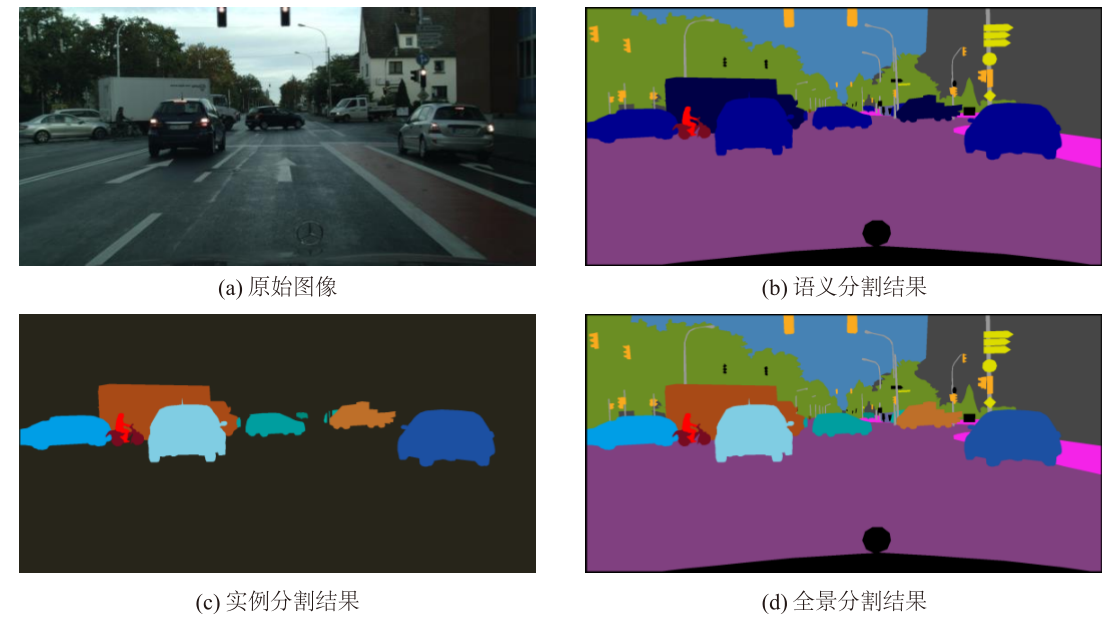
\includegraphics[width=8cm]{fig/chap1/全景分割1.png}
    \caption{不同种类分割示意图}
    \label{fig:f1a}
\end{figure}

全景分割是将语义分割和实例分割结合起来,以检测和分割图像中的所有物体和背景\cite{liu2020deep}。最初,全景分割采用了先检测后分割的方法,导致了自顶向下的双阶段方法的出现。例如,JSIS-Net、Panoptic FPN、EfficientPS和Auto-Panoptic等算法都使用第二阶段网络对第一阶段生成的候选区域进行后处理\cite{li2018detnet}。在对象检测过程中,常常需要使用第二阶段网络对第一阶段生成的候选区域进行后处理。然而,在后处理融合过程中,可能会出现语义分支与实例分支之间以及各分支内部的冲突。为了解决这个问题,研究人员提出了多种算法。例如,Liu等人提出的OANet利用注意力机制融合语义分支和实例分支,从而提高了对象检测的性能\cite{li2017fully}。Lazarow等人提出的OCFusion则使用多个分支处理不同的信息,并使用融合模块将它们合并在一起\cite{wang2018pelee}。此外,Yang等人提出的SOGNet利用基于分割的对象检测器,并同时融合了语义分支和实例分支\cite{chen2018searching}。这些算法的共同点是它们都通过第二阶段网络对第一阶段生成的候选区域进行后处理。然而,它们在解决语义分支与实例分支之间以及各分支内部冲突的方法上有所不同。在分支融合的基础上,Yang等人提出了BGRNet,其利用分支信息的互补性来实现对图像的全面理解。



\section{工作内容}
全景分割是一项具有挑战性和重要性的视觉任务,其关键难点是如何平衡分割效率和分割精度。在实际应用中,除了需要高精度的场景分割能力,还需要网络具备高效的运行效率。当前的全景分割方法通过后处理融合过程实现准确的全景分割,但这个过程耗时较长,无法满足实时运行的需求。此外,全景分割任务面临着复杂的场景,导致大尺度物体过度分割和小尺度物体分割不足的问题。为了解决这些问题,本研究专注于深度学习全景分割领域中的分支冲突、多尺度、实时性和准确性平衡等问题。通过感知像素级别的全景分割方法,旨在提高分割精度并保持高效的运行速度,以解决多尺度物体过度分割或分割不足的问题。网络推理过程简单明了,可通过深度学习推理引擎进行优化,从而降低在实际应用场景中的部署难度\cite{chandan2018real}。本文在Cityscapes公开标准数据集上与目前主流的全景分割方法进行了比较,并分析了本方法在分割性能上的优势。
